\section{Segment Everything Everywhere All at Once (SEEM)}
\begin{frame}{}
    \LARGE \textbf{Segment Everything Everywhere All at Once (SEEM)}
\end{frame}

\begin{frame}[allowframebreaks]{Segment Everything Everywhere All at Once (SEEM)}

\begin{center}
    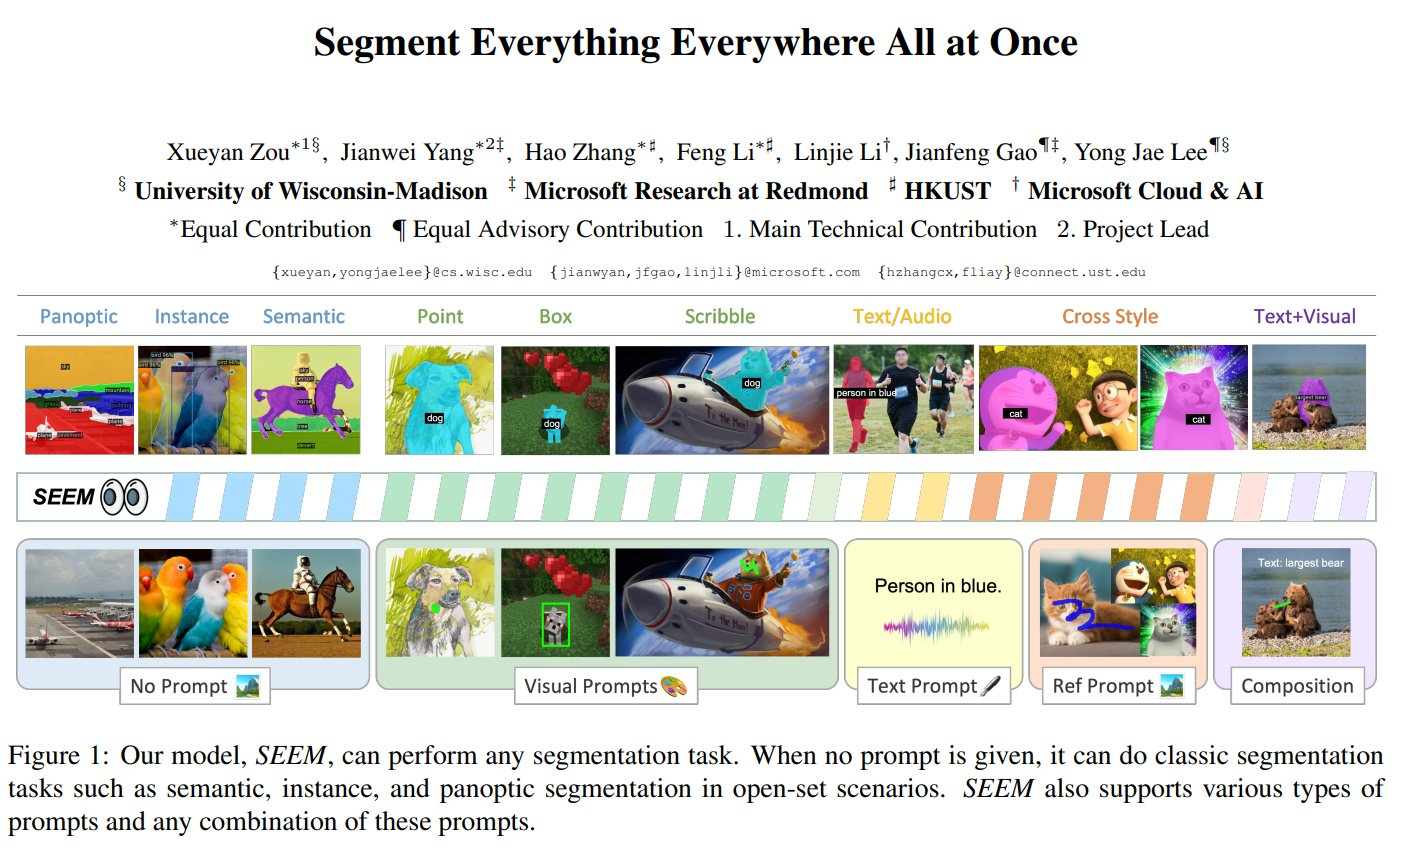
\includegraphics[width=\textwidth,height=0.9\textheight]{images/recent-advance/seem-paper.png}
\end{center}

\framebreak

\textbf{Proposed by Meta AI (2023)}

SEEM is a promptable panoptic segmentation model designed to segment any region, object, or stuff in an image using various input modalities such as text, points, boxes, or masks.

\begin{itemize}
    \item \textbf{Unified Segmentation:} Supports instance, semantic, and panoptic segmentation.
    \item \textbf{Versatility:} Works with any image, any resolution, and enables zero-shot segmentation.
    \item \textbf{Multimodal Prompts:} Accepts prompts in multiple forms, including text, points, boxes, and masks.
    \item \textbf{Video and Open Vocabulary:} Capable of segmenting video frames and handling open vocabulary tasks.
    \item \textbf{Foundation for Interactive Systems:} Serves as a foundation for real-time, interactive vision systems.
\end{itemize}

\framebreak

\begin{center}
    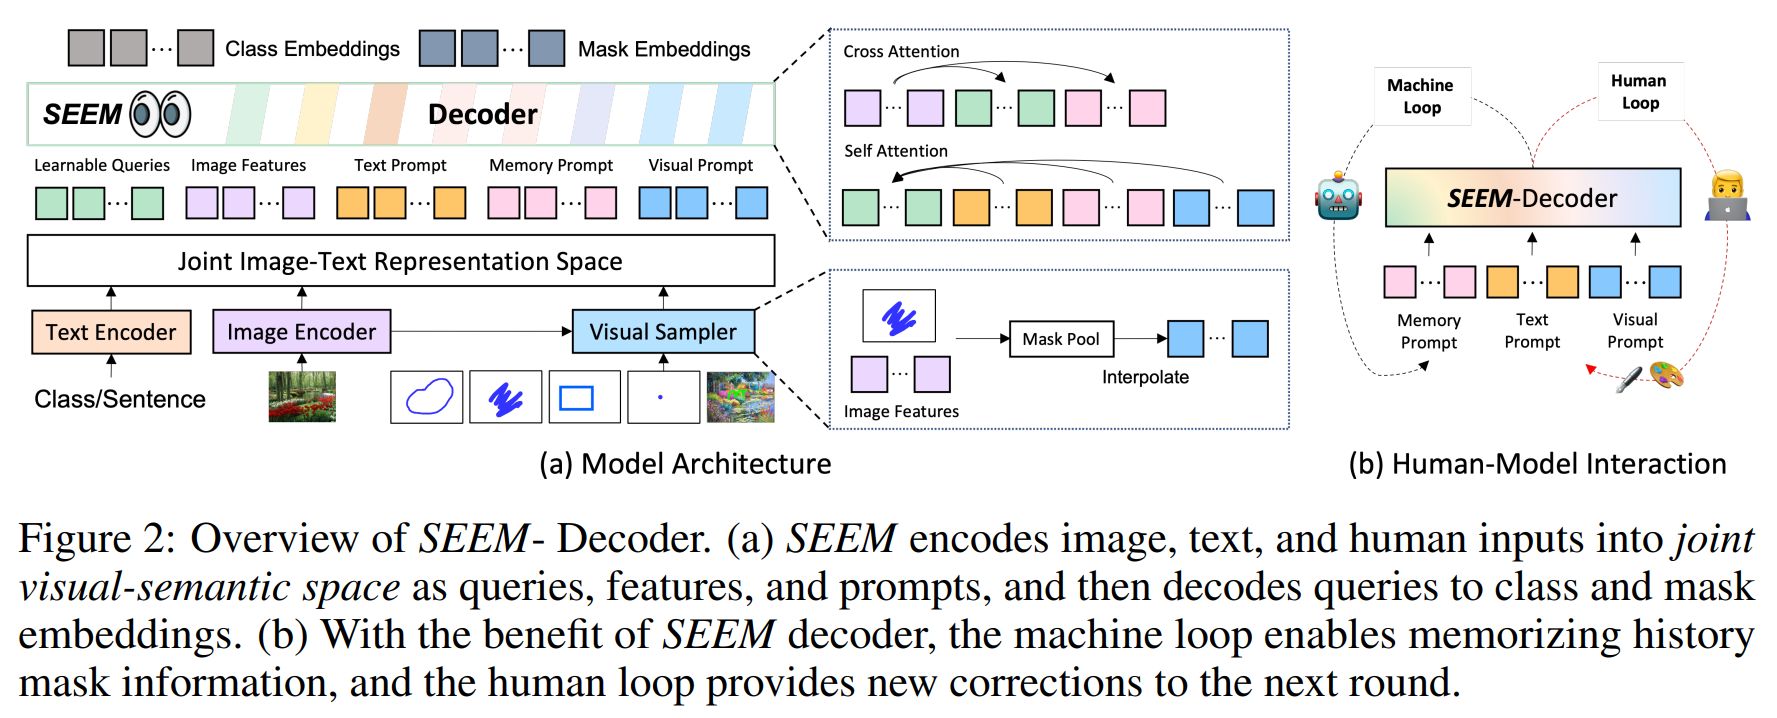
\includegraphics[width=\textwidth,height=0.9\textheight,keepaspectratio]{images/recent-advance/seem-overview.png}
\end{center}

\framebreak

\begin{center}
    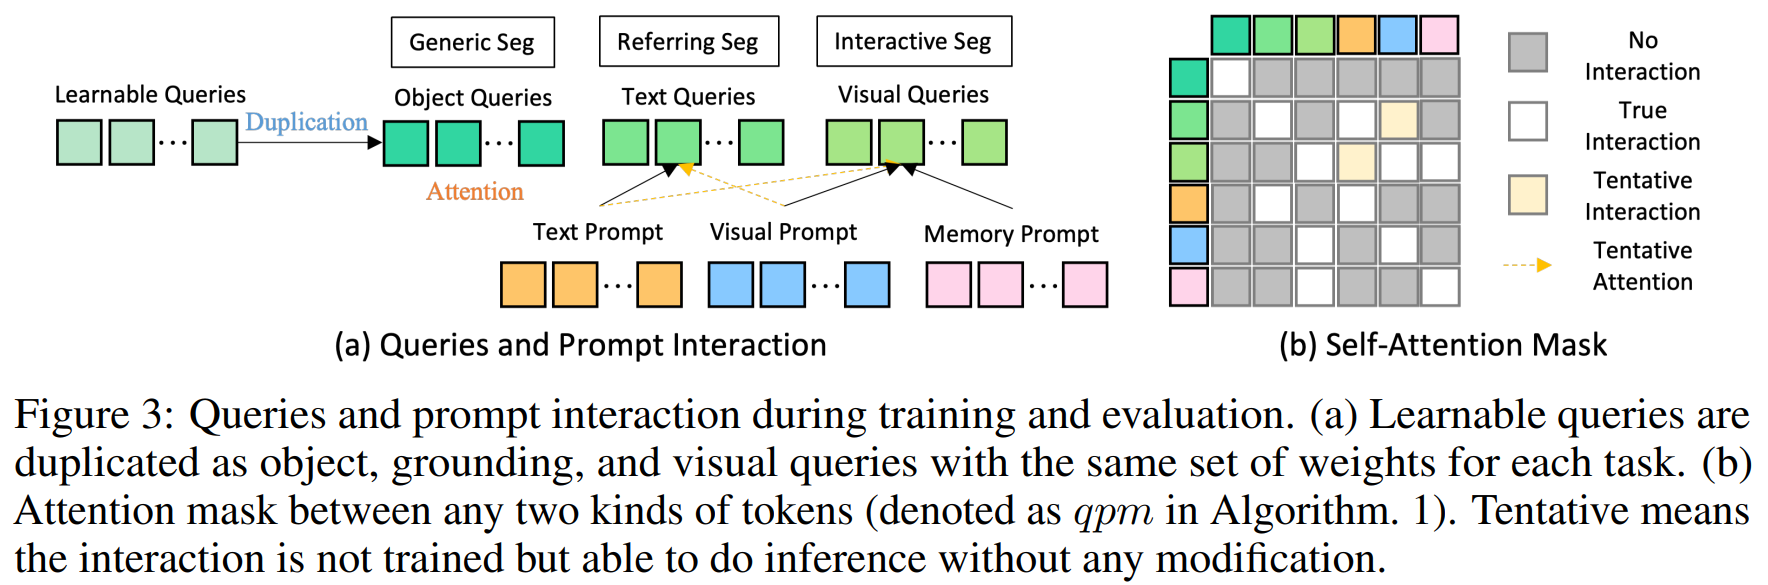
\includegraphics[width=\textwidth,height=0.9\textheight,keepaspectratio]{images/recent-advance/seem-query-prompt.png}
\end{center}

\framebreak

\begin{center}
    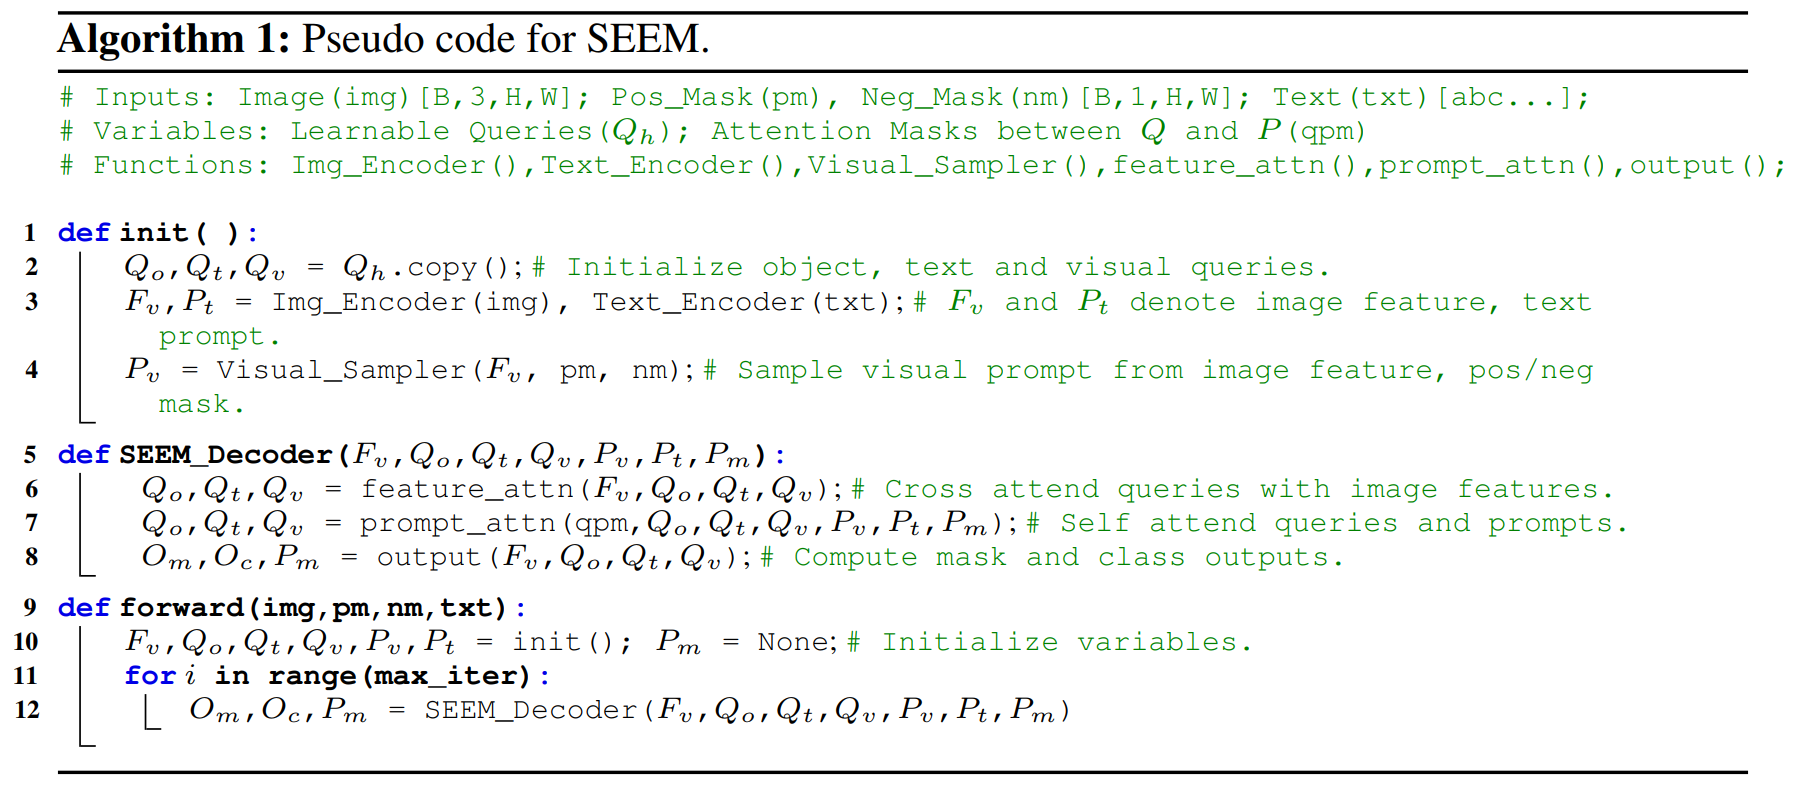
\includegraphics[width=1.085\textwidth,height=0.9\textheight,keepaspectratio]{images/recent-advance/seem-pseudocode.png}
\end{center}
\end{frame}


\begin{frame}[allowframebreaks]{SEEM - Results}
    \foreach \i in {1,...,4} { % Integers from 1 to 4
        \begin{figure}
            \centering
            \includegraphics[height=0.9\textheight,width=1\textwidth,keepaspectratio]{images/recent-advance/seem-result-\i.png}
        \end{figure}

        \framebreak
    }
\end{frame}